\documentclass[twoside]{book}

% Packages required by doxygen
\usepackage{fixltx2e}
\usepackage{calc}
\usepackage{doxygen}
\usepackage[export]{adjustbox} % also loads graphicx
\usepackage{graphicx}
\usepackage[utf8]{inputenc}
\usepackage{makeidx}
\usepackage{multicol}
\usepackage{multirow}
\PassOptionsToPackage{warn}{textcomp}
\usepackage{textcomp}
\usepackage[nointegrals]{wasysym}
\usepackage[table]{xcolor}

% Font selection
\usepackage[T1]{fontenc}
\usepackage[scaled=.90]{helvet}
\usepackage{courier}
\usepackage{amssymb}
\usepackage{sectsty}
\renewcommand{\familydefault}{\sfdefault}
\allsectionsfont{%
  \fontseries{bc}\selectfont%
  \color{darkgray}%
}
\renewcommand{\DoxyLabelFont}{%
  \fontseries{bc}\selectfont%
  \color{darkgray}%
}
\newcommand{\+}{\discretionary{\mbox{\scriptsize$\hookleftarrow$}}{}{}}

% Page & text layout
\usepackage{geometry}
\geometry{%
  a4paper,%
  top=2.5cm,%
  bottom=2.5cm,%
  left=2.5cm,%
  right=2.5cm%
}
\tolerance=750
\hfuzz=15pt
\hbadness=750
\setlength{\emergencystretch}{15pt}
\setlength{\parindent}{0cm}
\setlength{\parskip}{3ex plus 2ex minus 2ex}
\makeatletter
\renewcommand{\paragraph}{%
  \@startsection{paragraph}{4}{0ex}{-1.0ex}{1.0ex}{%
    \normalfont\normalsize\bfseries\SS@parafont%
  }%
}
\renewcommand{\subparagraph}{%
  \@startsection{subparagraph}{5}{0ex}{-1.0ex}{1.0ex}{%
    \normalfont\normalsize\bfseries\SS@subparafont%
  }%
}
\makeatother

% Headers & footers
\usepackage{fancyhdr}
\pagestyle{fancyplain}
\fancyhead[LE]{\fancyplain{}{\bfseries\thepage}}
\fancyhead[CE]{\fancyplain{}{}}
\fancyhead[RE]{\fancyplain{}{\bfseries\leftmark}}
\fancyhead[LO]{\fancyplain{}{\bfseries\rightmark}}
\fancyhead[CO]{\fancyplain{}{}}
\fancyhead[RO]{\fancyplain{}{\bfseries\thepage}}
\fancyfoot[LE]{\fancyplain{}{}}
\fancyfoot[CE]{\fancyplain{}{}}
\fancyfoot[RE]{\fancyplain{}{\bfseries\scriptsize Generated by Doxygen }}
\fancyfoot[LO]{\fancyplain{}{\bfseries\scriptsize Generated by Doxygen }}
\fancyfoot[CO]{\fancyplain{}{}}
\fancyfoot[RO]{\fancyplain{}{}}
\renewcommand{\footrulewidth}{0.4pt}
\renewcommand{\chaptermark}[1]{%
  \markboth{#1}{}%
}
\renewcommand{\sectionmark}[1]{%
  \markright{\thesection\ #1}%
}

% Indices & bibliography
\usepackage{natbib}
\usepackage[titles]{tocloft}
\setcounter{tocdepth}{3}
\setcounter{secnumdepth}{5}
\makeindex

% Hyperlinks (required, but should be loaded last)
\usepackage{ifpdf}
\ifpdf
  \usepackage[pdftex,pagebackref=true]{hyperref}
\else
  \usepackage[ps2pdf,pagebackref=true]{hyperref}
\fi
\hypersetup{%
  colorlinks=true,%
  linkcolor=blue,%
  citecolor=blue,%
  unicode%
}

% Custom commands
\newcommand{\clearemptydoublepage}{%
  \newpage{\pagestyle{empty}\cleardoublepage}%
}

\usepackage{caption}
\captionsetup{labelsep=space,justification=centering,font={bf},singlelinecheck=off,skip=4pt,position=top}

%===== C O N T E N T S =====

\begin{document}

% Titlepage & ToC
\hypersetup{pageanchor=false,
             bookmarksnumbered=true,
             pdfencoding=unicode
            }
\pagenumbering{alph}
\begin{titlepage}
\vspace*{7cm}
\begin{center}%
{\Large Robotic Football All In Many }\\
\vspace*{1cm}
{\large Generated by Doxygen 1.8.14}\\
\end{center}
\end{titlepage}
\clearemptydoublepage
\pagenumbering{roman}
\tableofcontents
\clearemptydoublepage
\pagenumbering{arabic}
\hypersetup{pageanchor=true}

%--- Begin generated contents ---
\chapter{Robotic-\/\+Football-\/\+All-\/\+In-\/\+Many}
\label{md__r_e_a_d_m_e}
\Hypertarget{md__r_e_a_d_m_e}
This is the multi-\/file code for the robotic football team. The design philosophy behind this project is to divide the code amoung a number of classes file to make it easy to maintain and share code between robots. The abilities of the robot to be programmed are then chosen from a list of define statements in \mbox{\hyperlink{_config_8hpp_source}{config.\+hpp}}, like so\+:

In \mbox{\hyperlink{_config_8hpp_source}{config.\+hpp}}\+: 
\begin{DoxyCode}
\{c++\}
//#define BASIC\_DRIVETRAIN
#define OMNIWHEEL\_DRIVETRAIN
//#define CENTER\_PERIPHERALS
#define QB\_PERIPHERALS
//#define KICKER\_PERIPHERALS
//#define RECEIVER\_PERIPHERALS
#define LED\_STRIP
#define TACKLE
\end{DoxyCode}
 This example would create a robot that uses an omniwheel drivetrain (specifically our quarterback), with the led strip and tackle sensor enabled. At the end of the file are a list of error cases that the compile goes through to make sure no incompatable options are shown.

\subsection*{\#\#\#\# Useful Libraries }


\begin{DoxyEnumerate}
\item (P\+S3 Integration) \href{https://github.com/felis/USB_Host_Shield_2.0}{\tt U\+SB Host\+Shield 2.\+0}
\item (Omniwheel Rotation Locking) \href{https://github.com/adafruit/Adafruit_BNO055}{\tt Adafruit B\+N\+O055}
\item (S\+TL for arduino) \href{https://github.com/maniacbug/StandardCplusplus}{\tt Standard\+Cplusplus}
\end{DoxyEnumerate}

\subsection*{\#\#\#\# Controls }


\begin{DoxyItemize}
\item {\bfseries Basic Drivetrain}
\begin{DoxyItemize}
\item {\itshape Up/\+Down Left Joystick} -\/ Forward and Backward movement
\item {\itshape Left/\+Right Right Joystick} -\/ Turning
\item {\itshape R2} -\/ activates \char`\"{}boost\char`\"{}
\item {\itshape Start} -\/ Puts robot in \char`\"{}kids mode\char`\"{}. The speed is reduced, boost is disabled, and the leds will change
\item {\itshape Select \+\_\+-\/ Calibration mode -\/ disables drivetrain while changes are made
\begin{DoxyItemize}
\item \+\_\+\+Up/\+Down D-\/\+Pad -\/ compensates for drag left or right
\item {\itshape Select} -\/ exit Calibration Mode to regular drive mode
\end{DoxyItemize}}
\end{DoxyItemize}
\item {\itshape {\bfseries \mbox{\hyperlink{class_center}{Center}}}
\begin{DoxyItemize}
\item \mbox{\hyperlink{class_center}{Center}} currently uses basic drivetrain
\item {\itshape T\+R\+I\+A\+N\+G\+LE} -\/ raise the center release servo
\item {\itshape C\+R\+O\+SS} -\/ lower the center release servo
\end{DoxyItemize}}
\item {\itshape {\bfseries Omniwheel Drivetrain}
\begin{DoxyItemize}
\item {\itshape Up/\+Down/\+Left/\+Right Left Joystick} -\/ Lateral movement in any direction
\item {\itshape Up/\+Down/\+Left/\+Right D-\/\+Pad}-\/ Lateral Movement along compass directions at full power
\item {\itshape Left/\+Right Right Joystick} -\/ Turning -\/ as of version 1.\+0.\+3 this will disable rotation correction
\item {\itshape R3} (Right Joystick Press) -\/ Re-\/engage rotation correction
\item {\itshape R2} -\/ slow down speed
\item {\itshape L1} -\/ reverse directions (make back of robot front and vise versa)
\item Throwing
\begin{DoxyItemize}
\item {\itshape S\+Q\+U\+A\+RE} -\/ Handoff throw
\item {\itshape C\+R\+O\+SS} -\/ Reciever handoff throw/weak toss
\item {\itshape C\+I\+R\+C\+LE} -\/ mid range throw
\item {\itshape T\+R\+I\+A\+N\+G\+LE} -\/ max power throw
\item {\itshape R1} -\/ return thrower to down position
\item {\itshape L2} -\/ hold to enable throw offset
\begin{DoxyItemize}
\item {\itshape Up/\+Down D-\/\+Pad} -\/ adjust power of all throws but triangle
\end{DoxyItemize}
\end{DoxyItemize}
\end{DoxyItemize}}
\item {\itshape {\bfseries \mbox{\hyperlink{class_kicker}{Kicker}}}
\begin{DoxyItemize}
\item \mbox{\hyperlink{class_kicker}{Kicker}} -\/ currently uses basic drivetrain
\item {\itshape C\+R\+O\+SS} -\/ kick
\item {\itshape T\+R\+I\+A\+N\+G\+LE} -\/ reload 
\end{DoxyItemize}}
\end{DoxyItemize}
\chapter{Module Index}
\section{Modules}
Here is a list of all modules\+:\begin{DoxyCompactList}
\item \contentsline{section}{Peripherals}{\pageref{group___peripherals}}{}
\item \contentsline{section}{Robot}{\pageref{group___robot}}{}
\item \contentsline{section}{Containers}{\pageref{group___containers}}{}
\item \contentsline{section}{Drive\+Train}{\pageref{group___drive_train}}{}
\end{DoxyCompactList}

\chapter{Class Index}
\section{Class List}
Here are the classes, structs, unions and interfaces with brief descriptions\+:\begin{DoxyCompactList}
\item\contentsline{section}{\mbox{\hyperlink{class_valpo_robotics_1_1array}{Valpo\+Robotics\+::array$<$ T, S\+I\+Z\+E $>$}} \\*Container that allows each member to be accessed in a range based for loop }{\pageref{class_valpo_robotics_1_1array}}{}
\item\contentsline{section}{\mbox{\hyperlink{class_basic_drive_controller}{Basic\+Drive\+Controller}} \\*This is the basic drivetrain that most robots use Used for most two motor robots }{\pageref{class_basic_drive_controller}}{}
\item\contentsline{section}{\mbox{\hyperlink{class_center}{Center}} \\*This class controls the centers dropper arm this class controlls the dropper arm that drops the football on a snap }{\pageref{class_center}}{}
\item\contentsline{section}{\mbox{\hyperlink{class_drive_train}{Drive\+Train}} \\*This class is the parent class for all other drive trains }{\pageref{class_drive_train}}{}
\item\contentsline{section}{\mbox{\hyperlink{class_drop_detector}{Drop\+Detector}} }{\pageref{class_drop_detector}}{}
\item\contentsline{section}{\mbox{\hyperlink{class_empty_peripheral}{Empty\+Peripheral}} }{\pageref{class_empty_peripheral}}{}
\item\contentsline{section}{\mbox{\hyperlink{class_kicker}{Kicker}} \\*This class controls the kicker peripheral }{\pageref{class_kicker}}{}
\item\contentsline{section}{\mbox{\hyperlink{class_l_e_d}{L\+ED}} \\*This class controls the robots L\+E\+Ds }{\pageref{class_l_e_d}}{}
\item\contentsline{section}{\mbox{\hyperlink{class_motor}{Motor}} }{\pageref{class_motor}}{}
\item\contentsline{section}{\mbox{\hyperlink{class_new_omni_drive}{New\+Omni\+Drive}} }{\pageref{class_new_omni_drive}}{}
\item\contentsline{section}{\mbox{\hyperlink{class_omni_drive_conrtoller}{Omni\+Drive\+Conrtoller}} \\*This is the drive train for omniwheel robots Used for most four motor robots }{\pageref{class_omni_drive_conrtoller}}{}
\item\contentsline{section}{\mbox{\hyperlink{class_peripheral}{Peripheral}} \\*This class is the parent class for all other drive trains }{\pageref{class_peripheral}}{}
\item\contentsline{section}{\mbox{\hyperlink{class_peripheral_name}{Peripheral\+Name}} \\*Provide an example }{\pageref{class_peripheral_name}}{}
\item\contentsline{section}{\mbox{\hyperlink{class_q_b_arm}{Q\+B\+Arm}} \\*This class controls the quaterback\textquotesingle{}s arm }{\pageref{class_q_b_arm}}{}
\item\contentsline{section}{\mbox{\hyperlink{class_robot}{Robot}} \\*Class that acts as a wrapper for other classes }{\pageref{class_robot}}{}
\item\contentsline{section}{\mbox{\hyperlink{class_tackle_seansor}{Tackle\+Seansor}} \\*This class controls the tackle sensor and its interaction with the L\+E\+Ds }{\pageref{class_tackle_seansor}}{}
\item\contentsline{section}{\mbox{\hyperlink{classtest_drive_conrtoller}{test\+Drive\+Conrtoller}} }{\pageref{classtest_drive_conrtoller}}{}
\end{DoxyCompactList}

\chapter{Module Documentation}
\hypertarget{group___peripherals}{}\section{Peripherals}
\label{group___peripherals}\index{Peripherals@{Peripherals}}

\hypertarget{group___robot}{}\section{Robot}
\label{group___robot}\index{Robot@{Robot}}
\subsection*{Classes}
\begin{DoxyCompactItemize}
\item 
class \mbox{\hyperlink{class_robot}{Robot}}
\begin{DoxyCompactList}\small\item\em Class that acts as a wrapper for other classes. \end{DoxyCompactList}\end{DoxyCompactItemize}


\subsection{Detailed Description}

\hypertarget{group___containers}{}\section{Containers}
\label{group___containers}\index{Containers@{Containers}}
\subsection*{Classes}
\begin{DoxyCompactItemize}
\item 
class \mbox{\hyperlink{class_valpo_robotics_1_1array}{Valpo\+Robotics\+::array$<$ T, S\+I\+Z\+E $>$}}
\begin{DoxyCompactList}\small\item\em container that allows each member to be accessed in a range based for loop \end{DoxyCompactList}\end{DoxyCompactItemize}


\subsection{Detailed Description}

\hypertarget{group___drive_train}{}\section{Drive\+Train}
\label{group___drive_train}\index{Drive\+Train@{Drive\+Train}}
\subsection*{Classes}
\begin{DoxyCompactItemize}
\item 
class \mbox{\hyperlink{class_basic_drive_controller}{Basic\+Drive\+Controller}}
\begin{DoxyCompactList}\small\item\em This is the basic drivetrain that most robots use Used for most two motor robots. \end{DoxyCompactList}\item 
class \mbox{\hyperlink{class_drive_train}{Drive\+Train}}
\begin{DoxyCompactList}\small\item\em This class is the parent class for all other drive trains. \end{DoxyCompactList}\item 
class \mbox{\hyperlink{class_omni_drive_conrtoller}{Omni\+Drive\+Conrtoller}}
\begin{DoxyCompactList}\small\item\em This is the drive train for omniwheel robots Used for most four motor robots. \end{DoxyCompactList}\end{DoxyCompactItemize}


\subsection{Detailed Description}

\chapter{Class Documentation}
\hypertarget{class_valpo_robotics_1_1array}{}\section{Valpo\+Robotics\+:\+:array$<$ T, S\+I\+ZE $>$ Class Template Reference}
\label{class_valpo_robotics_1_1array}\index{Valpo\+Robotics\+::array$<$ T, S\+I\+Z\+E $>$@{Valpo\+Robotics\+::array$<$ T, S\+I\+Z\+E $>$}}


container that allows each member to be accessed in a range based for loop  




{\ttfamily \#include $<$array.\+hpp$>$}

\subsection*{Public Member Functions}
\begin{DoxyCompactItemize}
\item 
\mbox{\Hypertarget{class_valpo_robotics_1_1array_ad1673d960bb1108221b2e5cb71dc1134}\label{class_valpo_robotics_1_1array_ad1673d960bb1108221b2e5cb71dc1134}} 
T $\ast$ \mbox{\hyperlink{class_valpo_robotics_1_1array_ad1673d960bb1108221b2e5cb71dc1134}{begin}} ()
\begin{DoxyCompactList}\small\item\em function that returns p\+Begin implemented so range based for loop will work \end{DoxyCompactList}\item 
\mbox{\Hypertarget{class_valpo_robotics_1_1array_a8b00881ddaed31c468e80020b275fe40}\label{class_valpo_robotics_1_1array_a8b00881ddaed31c468e80020b275fe40}} 
T $\ast$ \mbox{\hyperlink{class_valpo_robotics_1_1array_a8b00881ddaed31c468e80020b275fe40}{end}} ()
\begin{DoxyCompactList}\small\item\em function that returns p\+End implemented so range based for loop will work \end{DoxyCompactList}\item 
\mbox{\Hypertarget{class_valpo_robotics_1_1array_ab0d7f3c67b7928bd11b0fab2e5970d55}\label{class_valpo_robotics_1_1array_ab0d7f3c67b7928bd11b0fab2e5970d55}} 
void \mbox{\hyperlink{class_valpo_robotics_1_1array_ab0d7f3c67b7928bd11b0fab2e5970d55}{push\+\_\+back}} (T next\+Element)
\begin{DoxyCompactList}\small\item\em places an element in the next avaliable position if avaliable \end{DoxyCompactList}\end{DoxyCompactItemize}
\subsection*{Public Attributes}
\begin{DoxyCompactItemize}
\item 
\mbox{\Hypertarget{class_valpo_robotics_1_1array_a7769453fad25835d0cf35f577bc62faa}\label{class_valpo_robotics_1_1array_a7769453fad25835d0cf35f577bc62faa}} 
T \mbox{\hyperlink{class_valpo_robotics_1_1array_a7769453fad25835d0cf35f577bc62faa}{arr}} \mbox{[}S\+I\+ZE\mbox{]}
\begin{DoxyCompactList}\small\item\em underlying array \end{DoxyCompactList}\item 
\mbox{\Hypertarget{class_valpo_robotics_1_1array_a31464f62e42309a1ef2476910cade587}\label{class_valpo_robotics_1_1array_a31464f62e42309a1ef2476910cade587}} 
T $\ast$ \mbox{\hyperlink{class_valpo_robotics_1_1array_a31464f62e42309a1ef2476910cade587}{p\+Begin}} = \&(\mbox{\hyperlink{class_valpo_robotics_1_1array_a7769453fad25835d0cf35f577bc62faa}{arr}}\mbox{[}0\mbox{]})
\begin{DoxyCompactList}\small\item\em pointer to the start of the array \end{DoxyCompactList}\item 
\mbox{\Hypertarget{class_valpo_robotics_1_1array_a63deade950411259aa7a55a80b672cdf}\label{class_valpo_robotics_1_1array_a63deade950411259aa7a55a80b672cdf}} 
T $\ast$ \mbox{\hyperlink{class_valpo_robotics_1_1array_a63deade950411259aa7a55a80b672cdf}{p\+End}} = \mbox{\hyperlink{class_valpo_robotics_1_1array_a31464f62e42309a1ef2476910cade587}{p\+Begin}}
\begin{DoxyCompactList}\small\item\em pointer to the nex unused avaliable position in the array \end{DoxyCompactList}\end{DoxyCompactItemize}


\subsection{Detailed Description}
\subsubsection*{template$<$typename T, int S\+I\+ZE$>$\newline
class Valpo\+Robotics\+::array$<$ T, S\+I\+Z\+E $>$}

container that allows each member to be accessed in a range based for loop 

This container exists because std\+::array is unavaliable under arduino for no apparent reason. Do not use this in a non arduino context, use boost\+::array or std\+::array

\begin{DoxyNote}{Note}
Do not use this in a non arduino context.
\end{DoxyNote}
\begin{DoxyAuthor}{Author}
Bill Sullivan
\end{DoxyAuthor}
\begin{DoxyVersion}{Version}
\$\+Revision\+: 1.\+0
\end{DoxyVersion}
\begin{DoxyDate}{Date}
2018/08/14 14\+:16\+:20
\end{DoxyDate}
Created on\+: 2018/04/14 14\+:16\+:20 

The documentation for this class was generated from the following file\+:\begin{DoxyCompactItemize}
\item 
array.\+hpp\end{DoxyCompactItemize}

\hypertarget{class_peripheral}{}\section{Peripheral Class Reference}
\label{class_peripheral}\index{Peripheral@{Peripheral}}


This class is the parent class for all other drive trains.  




{\ttfamily \#include $<$Peripheral.\+hpp$>$}

Inheritance diagram for Peripheral\+:\begin{figure}[H]
\begin{center}
\leavevmode
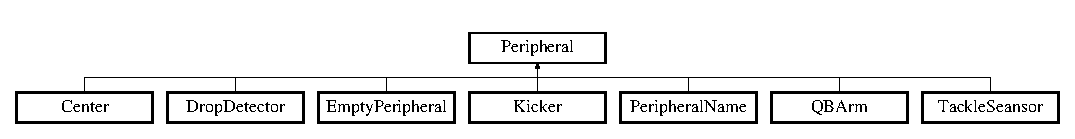
\includegraphics[height=1.651917cm]{class_peripheral}
\end{center}
\end{figure}
\subsection*{Public Member Functions}
\begin{DoxyCompactItemize}
\item 
\mbox{\Hypertarget{class_peripheral_adc231eaa2fec43878c139af159503727}\label{class_peripheral_adc231eaa2fec43878c139af159503727}} 
void \mbox{\hyperlink{class_peripheral_adc231eaa2fec43878c139af159503727}{do\+Not\+Connected\+Thing}} ()
\begin{DoxyCompactList}\small\item\em ensure the robot enters a safe state when connection to the controller is lost \end{DoxyCompactList}\item 
\mbox{\Hypertarget{class_peripheral_a5baf1180b80d1a61192542c29ae1d650}\label{class_peripheral_a5baf1180b80d1a61192542c29ae1d650}} 
void \mbox{\hyperlink{class_peripheral_a5baf1180b80d1a61192542c29ae1d650}{do\+Thing}} ()
\begin{DoxyCompactList}\small\item\em the implementation of do\+Thing should implement what happens when the controller is connected \end{DoxyCompactList}\item 
\mbox{\Hypertarget{class_peripheral_a3571b35c82ab213985cb1693be08904b}\label{class_peripheral_a3571b35c82ab213985cb1693be08904b}} 
void \mbox{\hyperlink{class_peripheral_a3571b35c82ab213985cb1693be08904b}{setup}} ()
\begin{DoxyCompactList}\small\item\em sets initial values of variables \end{DoxyCompactList}\end{DoxyCompactItemize}


\subsection{Detailed Description}
This class is the parent class for all other drive trains. 

This class is the parent class for all other drive trains

The only way this class should be used is as a parent class for other classes

\begin{DoxyAuthor}{Author}
Bill Sullivan
\end{DoxyAuthor}
\begin{DoxyVersion}{Version}
\$\+Revision\+: 1.\+0
\end{DoxyVersion}
\begin{DoxyDate}{Date}
2018/08/15 14\+:16\+:20
\end{DoxyDate}
Created on\+: 2018/04/14 14\+:16\+:20 

The documentation for this class was generated from the following file\+:\begin{DoxyCompactItemize}
\item 
Peripheral.\+hpp\end{DoxyCompactItemize}

\hypertarget{class_robot}{}\section{Robot Class Reference}
\label{class_robot}\index{Robot@{Robot}}


Class that acts as a wrapper for other classes.  




{\ttfamily \#include $<$Robot.\+hpp$>$}

\subsection*{Public Member Functions}
\begin{DoxyCompactItemize}
\item 
\mbox{\Hypertarget{class_robot_a1fc37e3c329d59795f6adf44199d4df9}\label{class_robot_a1fc37e3c329d59795f6adf44199d4df9}} 
void \mbox{\hyperlink{class_robot_a1fc37e3c329d59795f6adf44199d4df9}{setup}} ()
\begin{DoxyCompactList}\small\item\em Function that sets up the rest of the firmware setup function initilizes all variables sets up setial port to connect back to computer use to program the microcontroller. \end{DoxyCompactList}\item 
void \mbox{\hyperlink{class_robot_ad92e1e27045a02533f55ecab2b16d368}{loop}} ()
\begin{DoxyCompactList}\small\item\em Function that runs every to its end then repeats until device shutdown chekcs if controller is connectd if it is setup controller on first loop after connection then run drive train and peripheral\textquotesingle{}s connected code if it is not run drive train and peripheral\textquotesingle{}s not connected code. \end{DoxyCompactList}\end{DoxyCompactItemize}
\subsection*{Protected Member Functions}
\begin{DoxyCompactItemize}
\item 
void \mbox{\hyperlink{class_robot_aca73cd3e3582f49cc0b33ee900cbc245}{new\+Connection}} ()
\begin{DoxyCompactList}\small\item\em Function that runs when P\+S3 Controller connects. \end{DoxyCompactList}\end{DoxyCompactItemize}
\subsection*{Protected Attributes}
\begin{DoxyCompactItemize}
\item 
\mbox{\hyperlink{class_drive_train}{Drive\+Train}} $\ast$ \mbox{\hyperlink{class_robot_a4b499841182a38720a26a493fa98363a}{drive\+Train}}
\begin{DoxyCompactList}\small\item\em Pointer to an \mbox{\hyperlink{class_l_e_d}{L\+ED}}. \end{DoxyCompactList}\item 
\mbox{\hyperlink{class_valpo_robotics_1_1array}{Valpo\+Robotics\+::array}}$<$ \mbox{\hyperlink{class_peripheral}{Peripheral}} $\ast$, M\+A\+X\+\_\+\+T\+O\+T\+A\+L\+\_\+\+P\+E\+R\+I\+P\+E\+R\+A\+LS $>$ \mbox{\hyperlink{class_robot_a8db438771a3e7dc9d2cf5dd2e1d25f74}{peripheral\+Vec}}
\begin{DoxyCompactList}\small\item\em Array of pointers to Peripherals. \end{DoxyCompactList}\item 
\mbox{\Hypertarget{class_robot_a19c7a18705cf4bc4359f5ba12c3541d8}\label{class_robot_a19c7a18705cf4bc4359f5ba12c3541d8}} 
bool \mbox{\hyperlink{class_robot_a19c7a18705cf4bc4359f5ba12c3541d8}{newconnect}}
\begin{DoxyCompactList}\small\item\em variable that tracks if the controller is connected \end{DoxyCompactList}\end{DoxyCompactItemize}


\subsection{Detailed Description}
Class that acts as a wrapper for other classes. 

This class enables each peipheral and drivetrain to be run without having to know what the other peripherals are doing

\begin{DoxyNote}{Note}
Attempts at zen rarely work.
\end{DoxyNote}
\begin{DoxyAuthor}{Author}
Bill Sullivan
\end{DoxyAuthor}
\begin{DoxyVersion}{Version}
\$\+Revision\+: 1.\+0
\end{DoxyVersion}
\begin{DoxyDate}{Date}
2018/08/15 14\+:16\+:20
\end{DoxyDate}
Created on\+: 2018/04/14 14\+:16\+:20

\begin{DoxyParagraph}{Id}
doxygen-\/howto2.\+html,v 1.\+5 bv Exp 
\end{DoxyParagraph}


\subsection{Member Function Documentation}
\mbox{\Hypertarget{class_robot_ad92e1e27045a02533f55ecab2b16d368}\label{class_robot_ad92e1e27045a02533f55ecab2b16d368}} 
\index{Robot@{Robot}!loop@{loop}}
\index{loop@{loop}!Robot@{Robot}}
\subsubsection{\texorpdfstring{loop()}{loop()}}
{\footnotesize\ttfamily void Robot\+::loop (\begin{DoxyParamCaption}{ }\end{DoxyParamCaption})\hspace{0.3cm}{\ttfamily [inline]}}



Function that runs every to its end then repeats until device shutdown chekcs if controller is connectd if it is setup controller on first loop after connection then run drive train and peripheral\textquotesingle{}s connected code if it is not run drive train and peripheral\textquotesingle{}s not connected code. 

sets up setial port to connect back to computer use to program the microcontroller \mbox{\Hypertarget{class_robot_aca73cd3e3582f49cc0b33ee900cbc245}\label{class_robot_aca73cd3e3582f49cc0b33ee900cbc245}} 
\index{Robot@{Robot}!new\+Connection@{new\+Connection}}
\index{new\+Connection@{new\+Connection}!Robot@{Robot}}
\subsubsection{\texorpdfstring{new\+Connection()}{newConnection()}}
{\footnotesize\ttfamily void Robot\+::new\+Connection (\begin{DoxyParamCaption}{ }\end{DoxyParamCaption})\hspace{0.3cm}{\ttfamily [inline]}, {\ttfamily [protected]}}



Function that runs when P\+S3 Controller connects. 

Function that runs when P\+S3 Controller connects Function tells rest of the firmware and the user that the controller has connected 

\subsection{Member Data Documentation}
\mbox{\Hypertarget{class_robot_a4b499841182a38720a26a493fa98363a}\label{class_robot_a4b499841182a38720a26a493fa98363a}} 
\index{Robot@{Robot}!drive\+Train@{drive\+Train}}
\index{drive\+Train@{drive\+Train}!Robot@{Robot}}
\subsubsection{\texorpdfstring{drive\+Train}{driveTrain}}
{\footnotesize\ttfamily \mbox{\hyperlink{class_drive_train}{Drive\+Train}}$\ast$ Robot\+::drive\+Train\hspace{0.3cm}{\ttfamily [protected]}}



Pointer to an \mbox{\hyperlink{class_l_e_d}{L\+ED}}. 

Pointer to an \mbox{\hyperlink{class_l_e_d}{L\+ED}} Stores an pointer to an \mbox{\hyperlink{class_l_e_d}{L\+ED}} class so that all peipherals that acces the \mbox{\hyperlink{class_l_e_d}{L\+ED}} (ie the Tackle Sensor) access the same \mbox{\hyperlink{class_l_e_d}{L\+ED}} Pointer to a \mbox{\hyperlink{class_drive_train}{Drive\+Train}}

e\+Stop is run when the controller is disconnected do\+Thing runs continously when the controller is connected setup runs once when the microcontroller is turned on \mbox{\Hypertarget{class_robot_a8db438771a3e7dc9d2cf5dd2e1d25f74}\label{class_robot_a8db438771a3e7dc9d2cf5dd2e1d25f74}} 
\index{Robot@{Robot}!peripheral\+Vec@{peripheral\+Vec}}
\index{peripheral\+Vec@{peripheral\+Vec}!Robot@{Robot}}
\subsubsection{\texorpdfstring{peripheral\+Vec}{peripheralVec}}
{\footnotesize\ttfamily \mbox{\hyperlink{class_valpo_robotics_1_1array}{Valpo\+Robotics\+::array}}$<$\mbox{\hyperlink{class_peripheral}{Peripheral}}$\ast$, M\+A\+X\+\_\+\+T\+O\+T\+A\+L\+\_\+\+P\+E\+R\+I\+P\+E\+R\+A\+LS$>$ Robot\+::peripheral\+Vec\hspace{0.3cm}{\ttfamily [protected]}}



Array of pointers to Peripherals. 

do\+Not\+Connected\+Thing is run when the controller is disconnected do\+Thing runs continously when the controller is connected setup runs once when the microcontroller is turned on 

The documentation for this class was generated from the following file\+:\begin{DoxyCompactItemize}
\item 
Robot.\+hpp\end{DoxyCompactItemize}

%--- End generated contents ---

% Index
\backmatter
\newpage
\phantomsection
\clearemptydoublepage
\addcontentsline{toc}{chapter}{Index}
\printindex

\end{document}
